\section{状态与命令模式}

\subsection{状态模式}

\subsubsection{模式动机}
在很多情况下,\textbf{一个对象的行为取决于一个或多个动态变化的属性},这样的属性叫做\textbf{状态},这样的对象叫做有状态的(stateful)对象,这样的对象状态是从事先定义好的一系列值中取出的。当一个这样的对象与外部事件产生互动时,其内部状态就会改变 ,从而使得系统的行为也随之发生变化。

\subsubsection{模式定义}
状态模式(State Pattern):允许一个对象在其内部状态改变时改变它的行为,对象看起来似乎修改了它的类。其别名为状态对象(Objects for States),状态模式是一种对象行为型模式。

\subsubsection{模式结构}
状态模式包含如下角色:
\vspace{-0.8em}
\begin{multicols}{3}
    \begin{itemize}
        \item Context:环境类
        \item State:抽象状态类
        \item ConcreteState:具体状态类
    \end{itemize}
\end{multicols}
\vspace{-1em}

\begin{figure}[H]
    \vspace{-0.5em}
	\centering
	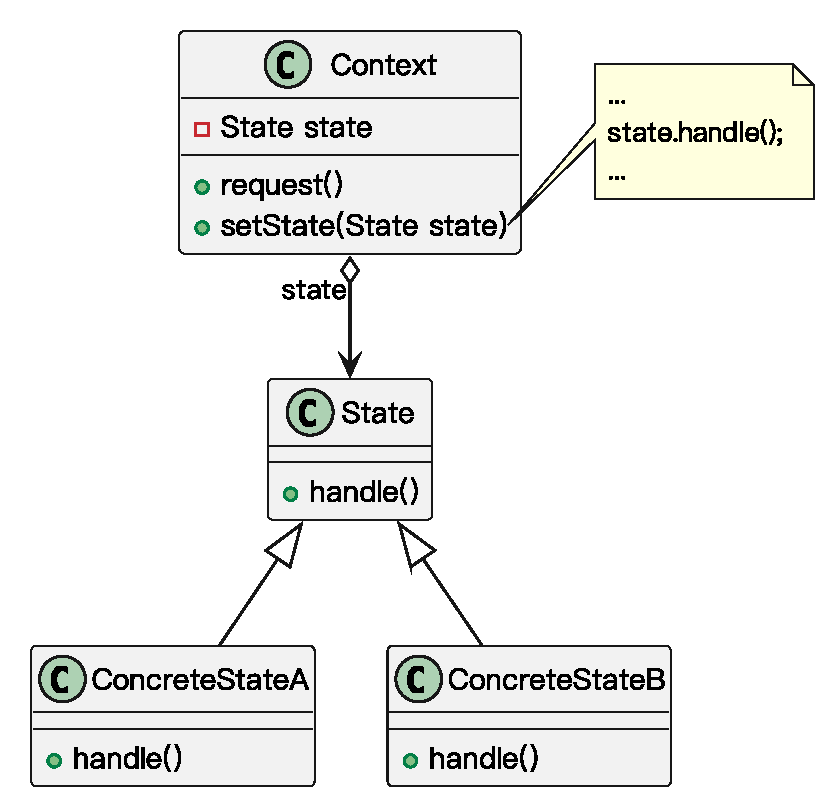
\includegraphics[width=0.42\textwidth]{images/状态模式结构.eps}
    \vspace{-1em}
\end{figure}

\subsubsection{模式分析}
\begin{figure}[H]
    \vspace{-0.5em}
	\centering
	\includegraphics[width=0.7\textwidth]{images/状态模式分析.pdf}
    \vspace{-1em}
\end{figure}

\begin{itemize}
    \item 状态模式描述了对象状态的变化以及对象如何在每一种状态下表现出不同的行为。
    \item 状态模式的关键是引入了一个抽象类来专门表示对象的状态,这个类我们叫做抽象状态类,而对象的每一种具体状态类都继承了该类,并在不同具体状态类中实现了不同状态的行为,包括各种状态之间的转换。
\end{itemize}

在状态模式结构中需要理解\textbf{环境类}与\textbf{抽象状态类}的作用:
\begin{itemize}
    \item 环境类实际上就是\textbf{拥有状态的对象},环境类有时候可以充当状态管理器(State Manager)的角色,\textbf{可以在环境类中对状态进行切换操作}。
    \item 抽象状态类可以是抽象类,也可以是接口,不同状态类就是继承这个父类的不同子类,状态类的产生是由于环境类存在多个状态,同时还满足两个条件:这些状态经常需要切换,在不同的状态下对象的行为不同。因此可以\textbf{将不同对象下的行为单独提取出来封装在具体的状态类中,使得环境类对象在其内部状态改变时可以改变它的行为,对象看起来似乎修改了它的类,而实际上是由于切换到不同的具体状态类实现的}。由于环境类可以设置为任一具体状态类,因此它针对抽象状态类进行编程,在程序运行时可以将任一具体状态类的对象设置到环境类中,从而使得环境类可以改变内部状态,并且改变行为。
\end{itemize}

\subsubsection{模式实例}
论坛用户等级:在某论坛系统中,用户可以发表留言,发表留言将增加积分;用户也可以回复留言,回复留言也将增加积分;用户还可以下载文件,下载文件将扣除积分。该系统用户分为三个等级,分别是新手、高手和专家,这三个等级对应三种不同的状态,这三种状态分别定义如下
\begin{enumerate}[label=(\arabic*)]
    \item 如果积分小于100分,则为新手状态,用户可以发表留言、回复留言,但是不能下载文件。如果积分大于等于1000分,则转换为专家状态;如果积分大于等于100分,则转换为高手状态。
    \item 如果积分大于等于100分但小于1000分,则为高手状态,用户可以发表留言、回复留言,还可以下载文件,而且用户在发表留言时可以获取双倍积分。如果积分小于100分,则转换为新手状态;如果积分大于等于1000分,则转换为专家状态;如果下载文件后积分小于0,则不能下载该文件。
    \item 如果积分大于等于1000分,则为专家状态,用户可以发表留言、回复留言和下载文件,用户除了在发表留言时可以获取双倍积分外,下载文件只扣除所需积分的一半。如果积分小于100分,则转换为新手状态;如果积分小于1000分,但大于等于100,则转换为高手状态;如果下载文件后积分小于0,则不能下载该文件。
\end{enumerate}
\begin{figure}[H]
    \vspace{-0.5em}
	\centering
	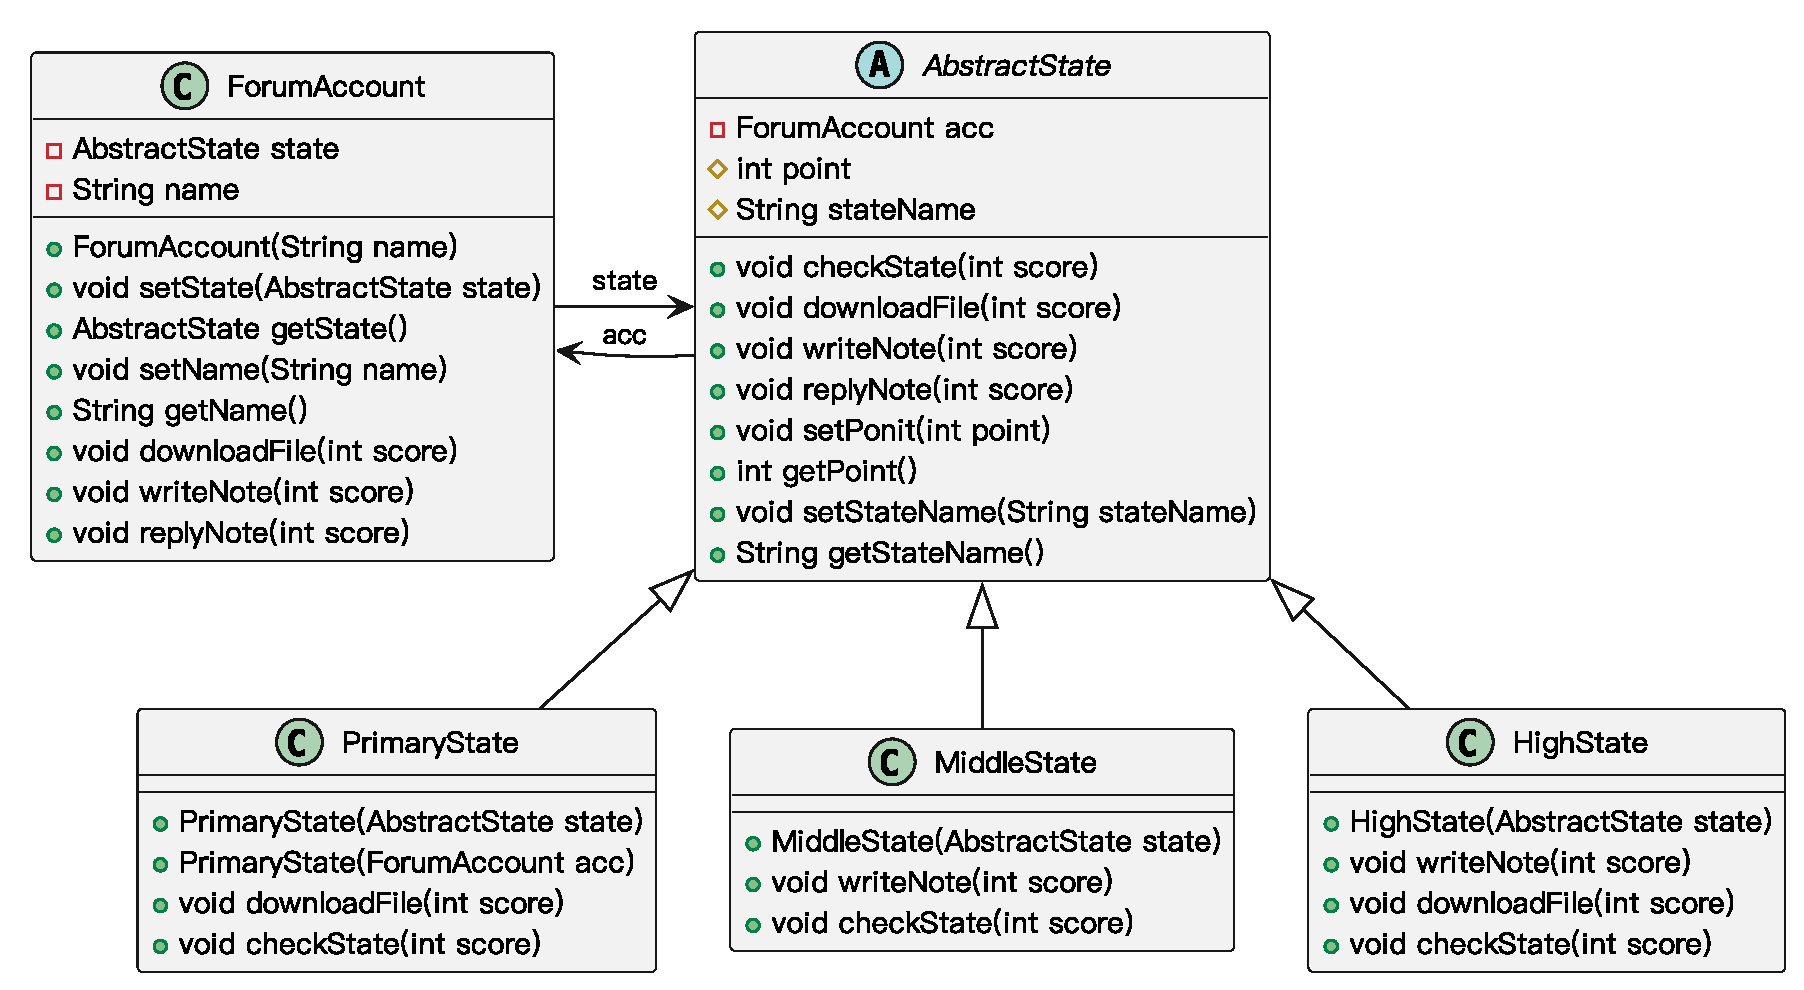
\includegraphics[width=0.8\textwidth]{images/状态模式实例.eps}
    \vspace{-1em}
\end{figure}

\subsubsection{模式优缺点}
状态模式的优点:
\begin{itemize}
    \item \textbf{封装了转换规则}。
    \item \textbf{枚举可能的状态},在枚举状态之前需要确定状态种类。
    \item 将所有与某个状态有关的行为放到一个类中,并且\textbf{可以方便地增加新的状态},只需要改变对象状态即可改变对象的行为。
    \item 允许\textbf{状态转换逻辑与状态对象合成一体},而不是某一个巨大的条件语句块。
    \item 可以\textbf{让多个环境对象共享一个状态对象},从而减少系统中对象的个数。
\end{itemize}

状态模式的缺点:
\begin{itemize}
    \item 状态模式的使用必然会\textbf{增加系统类和对象的个数}。
    \item 状态模式的结构与实现都较为复杂,\textbf{如果使用不当将导致程序结构和代码的混乱}。
    \item 状态模式\textbf{对“开闭原则”的支持并不太好},对于可以切换状态的状态模式,增加新的状态类需要修改那些负责状态转换的源代码,否则无法切换到新增状态;而且修改某个状态类的行为也需修改对应类的源代码。
\end{itemize}

\subsubsection{模式适用环境}
在以下情况下可以使用状态模式:
\begin{itemize}
    \item 对象的\textbf{行为依赖于它的状态(属性)}并且可以\textbf{根据它的状态改变而改变它的相关行为}。
    \item 代码中\textbf{包含大量与对象状态有关的条件语句},这些条件语句的出现,会导致代码的可维护性和灵活性变差,不能方便地增加和删除状态,使客户类与类库之间的耦合增强。在这些条件语句中包含了对象的行为,而且这些条件对应于对象的各种状态。
\end{itemize}

\subsubsection{模式应用}
\ding{172} 状态模式在\textbf{工作流}或\textbf{游戏}等类型的软件中得以广泛使用,甚至可以用于这些系统的核心功能设计,如在政府OA办公系统中,一个批文的状态有多种:尚未办理、正在办理、正在批示、正在审核、已经完成等各种状态,而且批文状态不同时对批文的操作也有所差异。\textbf{使用状态模式可以描述工作流对象(如批文)的状态转换以及不同状态下它所具有的行为}。

\ding{173} 在目前主流的RPG(角色扮演游戏)中,\textbf{使用状态模式可以对游戏角色进行控制},游戏角色的升级伴随着其状态的变化和行为的变化。对于游戏程序本身也可以通过状态模式进行总控,一个游戏活动包括开始、运行、结束等状态,通过对状态的控制可以控制系统的行为,决定游戏的各个方面,因此\textbf{可以使用状态模式对整个游戏的架构进行设计与实现}。

\subsubsection{模式扩展}

\paragraph*{共享状态}~{} \par
在有些情况下\textbf{多个环境对象需要共享同一个状态},如果希望在系统中实现多个环境对象实例共享一个或多个状态对象,那么\textbf{需要将这些状态对象定义为环境的静态成员对象}。

\paragraph*{简单状态模式}~{} \par
简单状态模式是指状态都相互独立,状态之间无须进行转换的状态模式,这是最简单的一种状态模式。
\begin{itemize}
    \item 对于这种状态模式,每个状态类都封装与状态相关的操作,而无须关心状态的切换,可以在客户端 直接实例化状态类,然后将状态对象设置到环境类中。
    \item 如果是这种简单的状态模式,它遵循“开闭原则”,在客户端可以针对抽象状态类进行编程,而将具体状态类写到配置文件中,同时增加新的状态类对原有系统也不造成任何影响。
\end{itemize} 

\paragraph*{可切换状态的状态模式}~{} \par
大多数的状态模式都是可以切换状态的状态模式
\begin{itemize}
    \item 在实现状态切换时,在具体状态类内部需要调用环境类\;\verb|Context的setState()|\;方法进行状态的转换操作,在具体状态类中可以调用到环境类的方法,因此状态类与环境类之间通常还存在关联关系或者依赖关系。
    \item 通过在状态类中引用环境类的对象来回调环境类的\;\verb|setState()|\;方法实现状态的切换。
    \item 在这种可以切换状态的状态模式中,增加新的状态类可能需要修改其他某些状态类甚至环境类的源代码,否则系统无法切换到新增状态。
\end{itemize}


\subsection{命令模式}

\subsubsection{模式动机}
在软件设计中,我们经常需要向某些对象发送请求,但是并不知道请求的接收者是谁,也不知道被请求的操作是哪个,我们只需在程序运行时指定具体的请求接收者即可,此时可以使用命令模式来进行设计,\textbf{使得请求发送者与请求接收者消除彼此之间的耦合},让对象之间的调用关系更加灵活。

命令模式可以对发送者和接收者完全解耦,发送者与接收者之间没有直接引用关系,\textbf{发送请求的对象只需要知道如何发送请求,而不必知道如何完成请求}。这就是命令模式的模式动机。

\subsubsection{模式定义}
命令模式(Command Pattern):将一个请求封装为一个对象,从而使我们可用不同的请求对客户进行参数化;对请求排队或者记录请求日志,以及支持可撤销的操作。命令模式是一种对象行为型模式,其别名为动作(Action)模式或事务(Transaction)模式。

\subsubsection{模式结构}
命令模式包含如下角色:
\vspace{-0.8em}
\begin{multicols}{2}
    \begin{itemize}
        \item Command: 抽象命令类
        \item ConcreteCommand: 具体命令类
        \item Invoker: 调用者
        \item Receiver: 接收者
        \item Client:客户类
    \end{itemize}
\end{multicols}
\vspace{-1em}
\begin{figure}[H]
    \vspace{-0.5em}
	\centering
	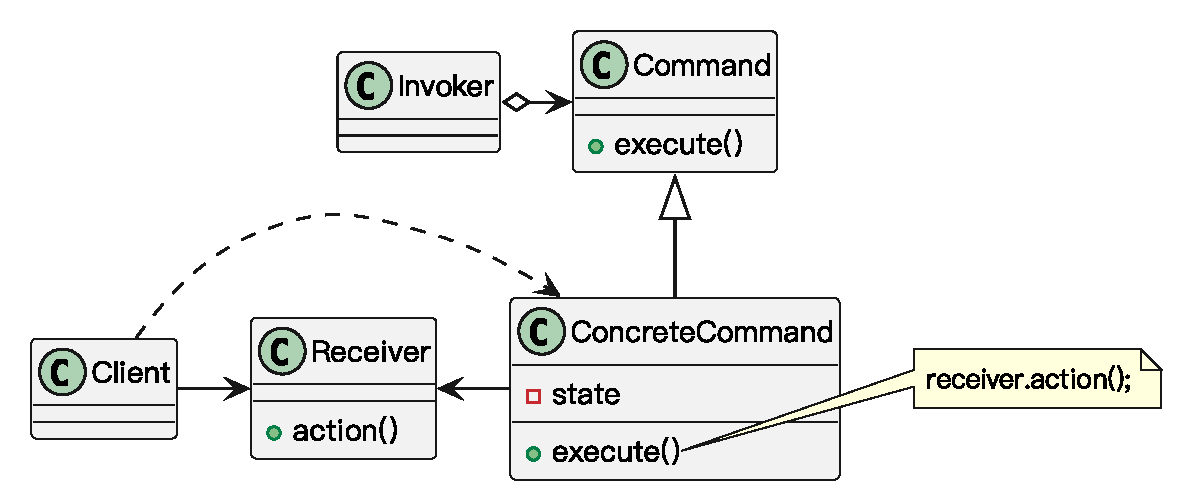
\includegraphics[width=0.65\textwidth]{images/命令模式结构.eps}
    \vspace{-1em}
\end{figure}

\subsubsection{模式分析}
\begin{itemize}
    \item 命令模式的本质是\textbf{对命令进行封装,将发出命令的责任和执行命令的责任分割开}。
    \item 每一个命令都是一个\textbf{操作}:请求的一方发出请求,要求执行一个操作;接收的一方收到请求,并执行操作。
    \item 命令模式允许请求的一方和接收的一方独立开来,使得\textbf{请求的一方不必知道接收请求的一方的接口},更不必知道请求是怎么被接收,以及操作是否被执行、何时被执行,以及是怎么被执行的。
    \item 命令模式\textbf{使请求本身成为一个对象},这个对象和其他对象一样可以被存储和传递。
    \item 命令模式的关键在于\textbf{引入了抽象命令接口},且\textbf{发送者针对抽象命令接口编程},只有实现了抽象命令接口的\textbf{具体命令才能与接收者相关联}。
\end{itemize}

命令模式顺序图
\begin{figure}[H]
    \vspace{-0.5em}
	\centering
	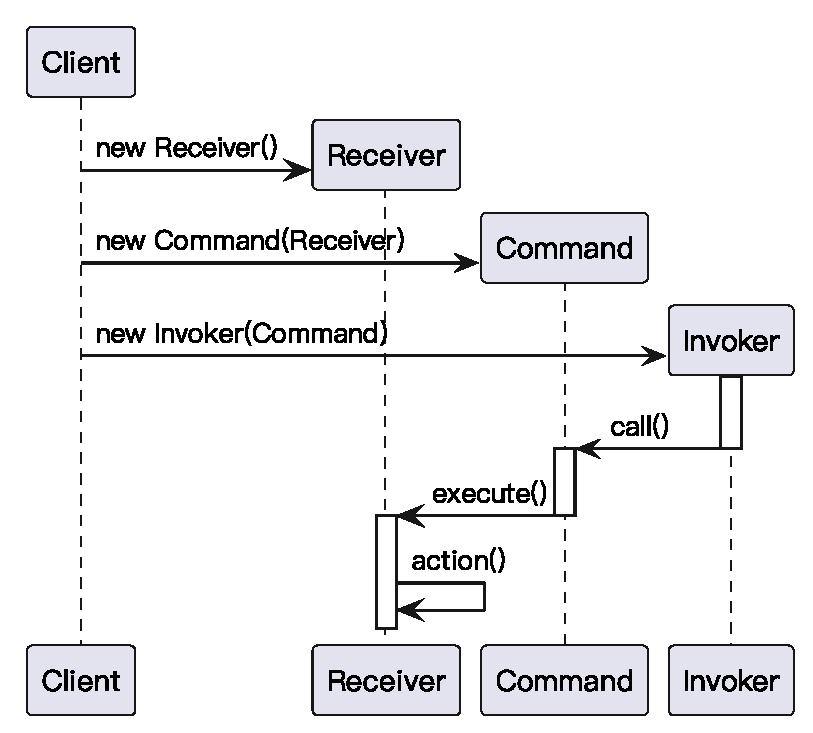
\includegraphics[width=0.5\textwidth]{images/命令模式顺序图.eps}
    \vspace{-1em}
\end{figure}

命令模式典型代码:
\begin{figure}[H]
    \vspace{-0.5em}
	\centering
	\includegraphics[width=0.75\textwidth]{images/命令模式典型代码.pdf}
    \vspace{-1em}
\end{figure}

\subsubsection{模式实例}
电视机遥控器:电视机是请求的接收者,遥控器是请求的发送者,遥控器上有一些按钮,不同的按钮对应电视机的不同操作。抽象命令角色由一个命令接口来扮演,有三个具体的命令类实现了抽象命令接口,这三个具体命令类分别代表三种操作:打开电视机、关闭电视机和切换频道。显然,电视机遥控器就是一个典型的命令模式应用实例。
\begin{figure}[H]
    \vspace{-0.5em}
	\centering
	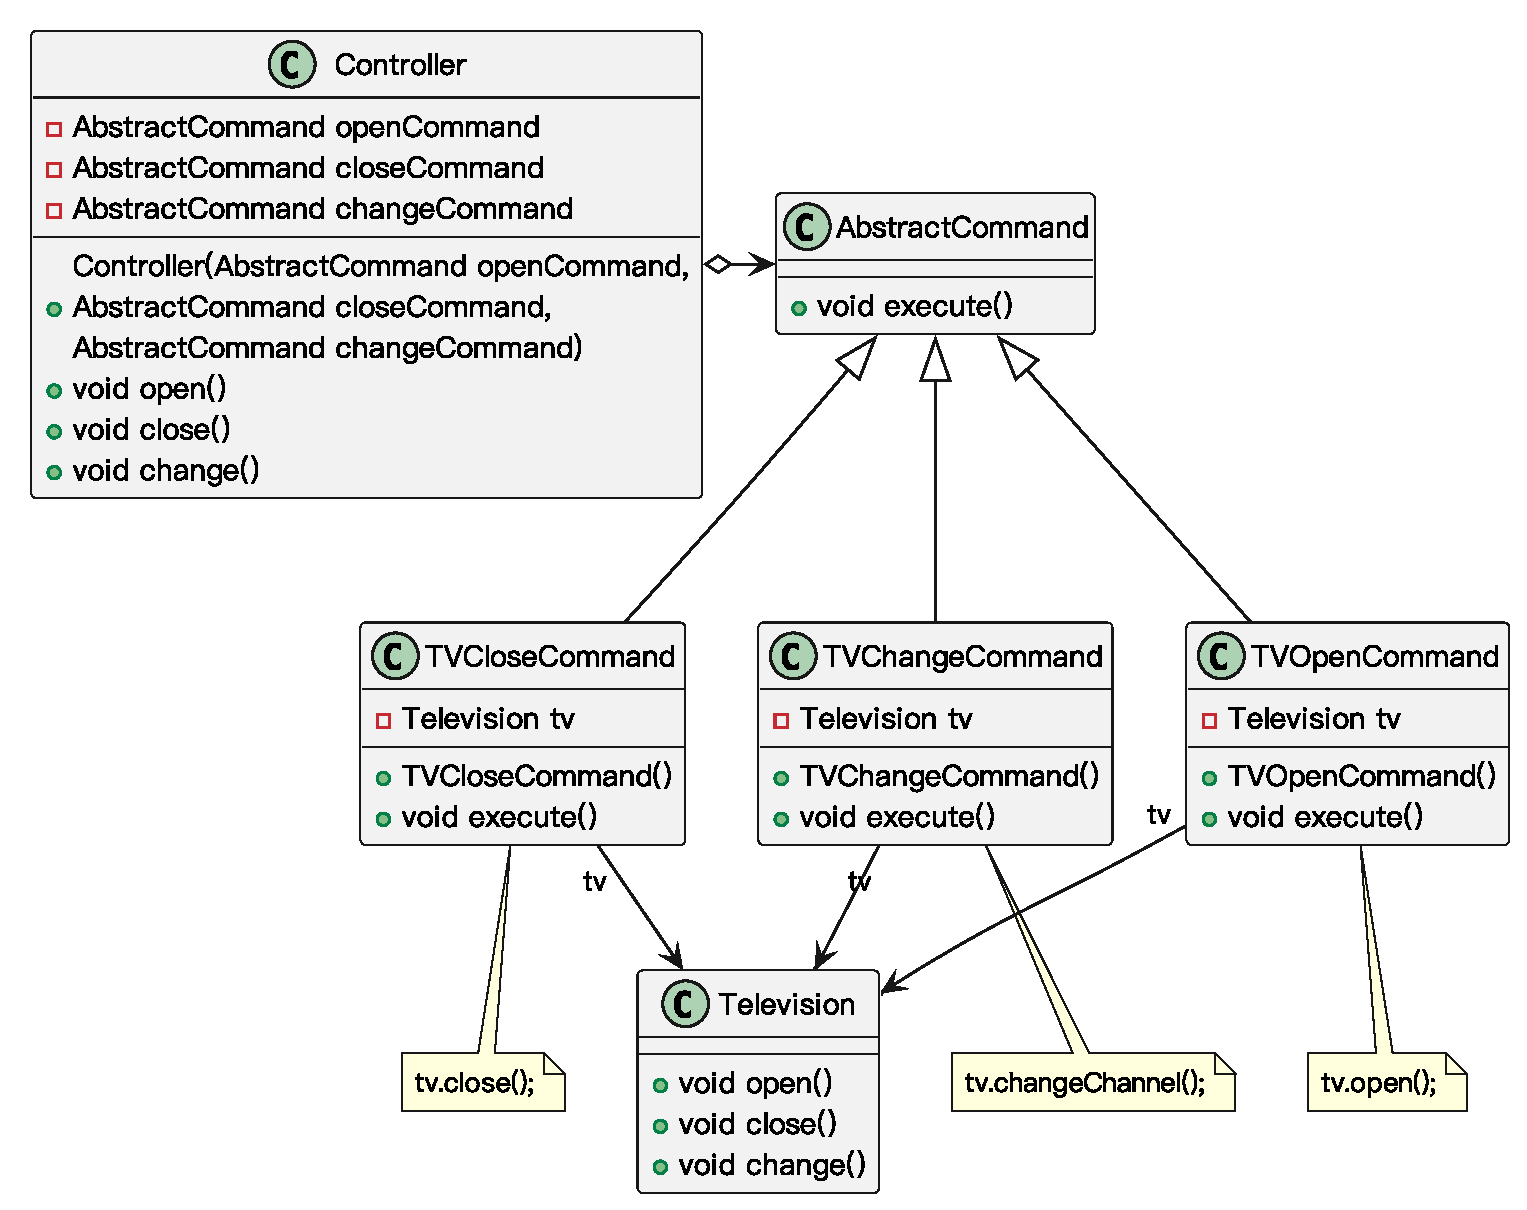
\includegraphics[width=0.85\textwidth]{images/命令模式实例1.eps}
    \vspace{-1em}
\end{figure}

功能键设置:为了用户使用方便,某系统提供了一系列功能键,用户可以自定义功能键的功能,如功能键FunctionButton可以用于退出系统(SystemExitClass),也可以用于打开帮助界面(DisplayHelpClass)。用户可以通过修改配置文件来改变功能键的用途,现使用命令模式来设计该系统,使得功能键类与功能类之间解耦,相同的功能键可以对应不同的功能。
\begin{figure}[H]
    \vspace{-0.5em}
	\centering
	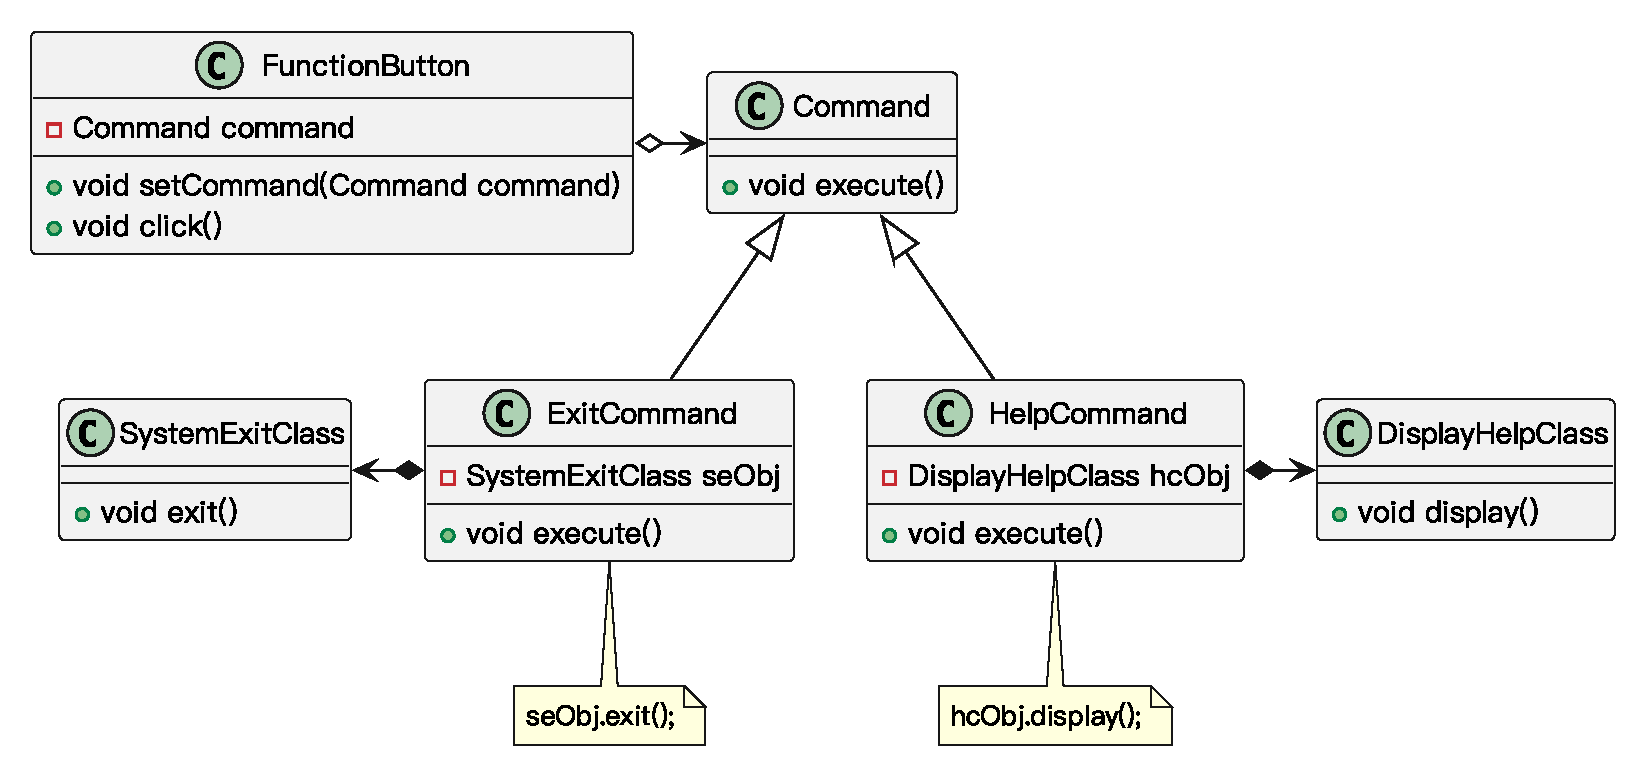
\includegraphics[width=0.85\textwidth]{images/命令模式实例2.eps}
    \vspace{-1em}
\end{figure}

\subsubsection{模式优缺点}
命令模式的优点:
\begin{itemize}
    \item 降低系统的耦合度。
    \item 新的命令可以很容易地加入到系统中。
    \item 可以比较容易地设计一个命令队列和宏命令(组合命令)。
    \item 可以方便地实现对请求的Undo和Redo。
\end{itemize}

命令模式的缺点:
\begin{itemize}
    \item 使用命令模式可能会\textbf{导致某些系统有过多的具体命令类}。因为针对每一个命令都需要设计一个具体命令类,因此某些系统可能需要大量具体命令类,这将影响命令模式的使用。
\end{itemize}

\subsubsection{模式适用环境}
在以下情况下可以使用命令模式:
\begin{itemize}
    \item 系统需要将请求调用者和请求接收者解耦,使得调用者和接收者不直接交互。
    \item 系统需要在不同的时间指定请求、将请求排队和执行请求。
    \item 系统需要支持命令的撤销(Undo)操作和恢复(Redo)操作。
    \item 系统需要将一组操作组合在一起,即支持宏命令。
\end{itemize}

\subsubsection{模式应用}
\ding{172} Java语言使用命令模式实现AWT/Swing GUI的委派事件模型 (Delegation Event Model, DEM) 。
\begin{itemize}
    \item 在AWT/Swing中,Frame、Button等界面组件是请求发送者,而AWT提供的事件监听器接口和事件适配器类是抽象命令接口,用户可以自己写抽象命令接口的子类来实现事件处理,即实现具体命令类,而在具体命令类中可以调用业务处理方法来实现该事件的处理。对于界面组件而言,只需要了解命令接口即可,无须关心接口的实现,组件类并不关心实际操作,而操作由用户来实现。
\end{itemize}

\ding{173} 很多系统都提供了宏命令功能,如Unix平台下的Shell编程,可以将多条命令封装在一个命令对象中,只需要一条简单的命令即可执行一个命令序列,这也是命令模式的应用实例之一。

\vspace{-0.5em}
\begin{shaded}
宏命令又称为组合命令,它是命令模式和组合模式联用的产物。

宏命令也是一个具体命令,不过它包含了对其他命令对象的引用,在调用宏命令的\;\verb|execute()|\;方法时,将递归调用 它所包含的每个成员命令的\;\verb|execute()|\;方法,一个宏命令 的成员对象可以是简单命令,还可以继续是宏命令。执行 一个宏命令将执行多个具体命令,从而实现对命令的批处 理。
\end{shaded}
\vspace{-1em}

\subsubsection{模式扩展}
撤销操作的实现
\begin{figure}[H]
    \vspace{-0.5em}
	\centering
	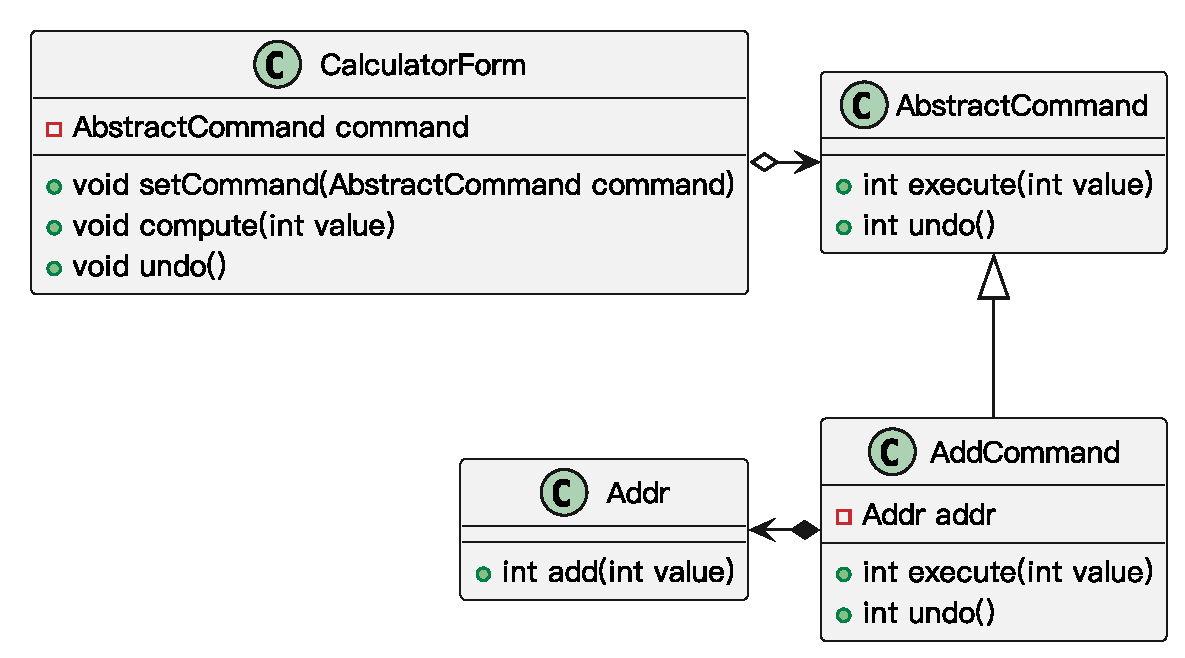
\includegraphics[width=0.7\textwidth]{images/命令模式拓展1.eps}
    \vspace{-1em}
\end{figure}

宏命令
\begin{figure}[H]
    \vspace{-0.5em}
	\centering
	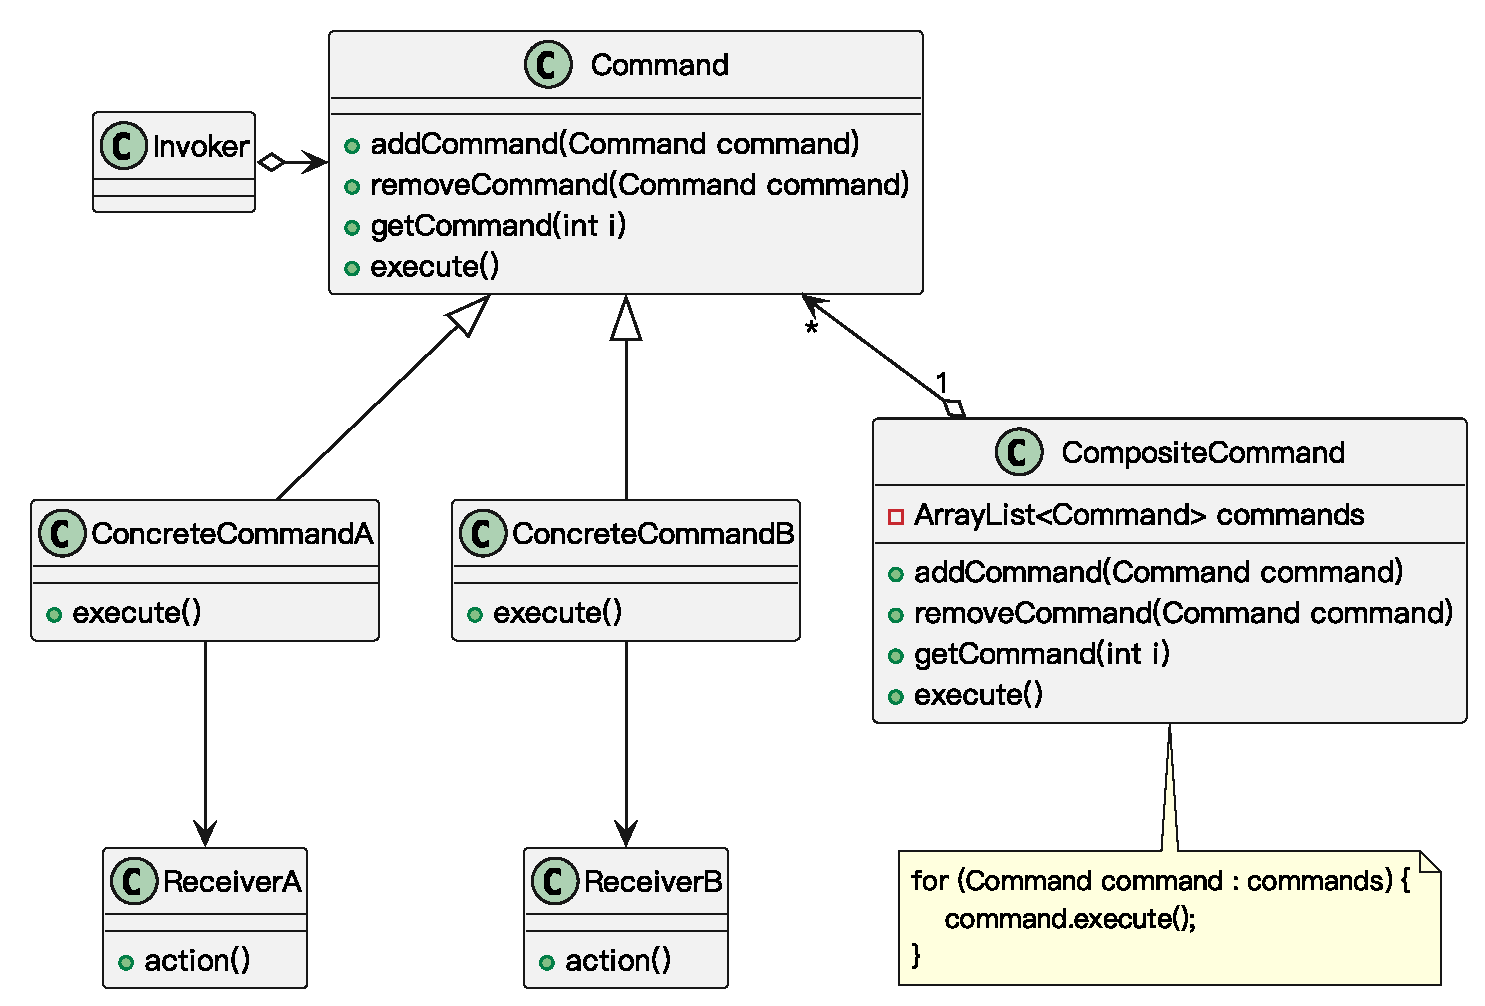
\includegraphics[width=0.8\textwidth]{images/命令模式拓展2.eps}
    \vspace{-1em}
\end{figure}